\chapter{A probléma megvalósítása}
\section{A felhasznált módszerek} \label{math_modells}
A probléma megoldására a következő, Hegyháti által kidolgozott \cite{phd_Hegyhati} módszerek adottak. Feladatom ezen módszerek tanulmányozása, és megértése után, ezek implementációja volt az S-gráf keretrendszerben.
\subsection{Preventív ütemezés fix batch mérettel}
Ebben az esetben az egyetlen döntés, amit meg kell hozni, hogy az egyes termékekből hány darab batch-et gyártsunk, a várható profit a következőképpen számítható ki:
$$\sum_{p \in P}\bigg (\sum_{s \in S} prob_s \cdot profit_{s,p} (s_p \cdot b_p)\bigg)$$
Érdemes még bevezetni adott $p$ termék $x$ értékben vett várható profit értékére a következő jelölést:
$$ExpProfit_p(x)=\sum_{s \in S}prob_s \cdot profit_{s,p}(x)$$
$ExpProfit_p(x)$ kiszámításához tehát nincs másra szükségünk, mint hogy az összes forgatókönyvre sorban felépítsünk az adott forgatókönyvre vonatkozó sztochasztikus paraméterekből a $profit_{s,p}$ függvényt, majd ezt a függvény beszorozzuk az aktuális $prob_s$ értékkel, amely lényegében a függvény "összenyomását" jelenti. Miután minden forgatókönyvre előállítottuk a \ref{profit_func_prob} ábrához hasonlóan ezt az "összenyomott" profit függvényt, ezen függvények összeadásával előáll az $ExpProfit_p$, ha ezt minden termékre megtesszük, az adott $p$ termékek $ExpProfit_p(x) \text{ (ahol }x=s_p \cdot b_p)$ értékének összegeként előáll a várható profit.
\begin{figure}[H]
\begin{center}
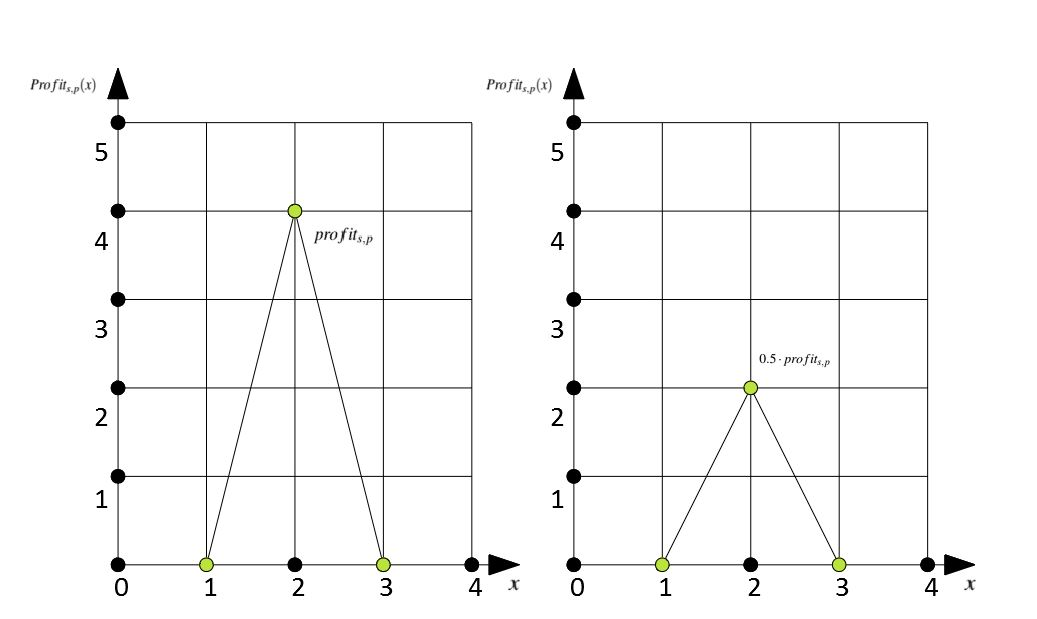
\includegraphics[scale=0.5]{profit_func_prob}
\caption{A profit függvény szorzásának szemléltetése}
\label{profit_func_prob}
\end{center}
\end{figure}
\subsection{Preventív ütemezés változó batch mérettel} \label{variable_batch_size_modell}
Az előző esettel ellentétben, változó batch méret esetén a batch darabszám nem határozza meg egyértelműen az adott termékből termelt mennyiséget. Ebben az esetben a batch méretről való döntés is a megoldó algoritmus feladata úgy, hogy $p$ termék batch mérete $s_p^{min}$ és $s_p^{max}$ között legyen. Mivel ezt a döntést előre meg kell hozni, ezért minden forgatókönyvben azonos méretű lesz minden $p$ termékhez tartozó batch. Ezután, már csak arról kell döntést hozni, hogy adott termékből mennyit gyártsunk, ez az $x_p$ érték a következő intervallumból kerül kiválasztásra: $[s_p^{min} \cdot b_p , s_p^{max} \cdot b_p]$. Az $ExpProfit$ függvény maximális értékét az egyik keresleti értékben veszi fel, legyen ez $dem_{s'}$. Az optimális $x_p$ érték kiválasztása a következőképpen tehető meg:
\begin{equation*}
x_{p}(b_p)= \begin{cases}
            b_p \cdot s_p^{max} \quad \text{ha } b_p \cdot s_p^{max}<dem_{s'}\\
            dem_{s'} \qquad \text{ha } b_p \cdot s_p^{min} \leq dem_{s'} \leq b_p \cdot s_p^{max}\\
            b_p \cdot s_p^{min} \quad \text{ ha } b_p \cdot s_p^{min}>dem_{s'}
       \end{cases}       
\end{equation*}\\
A \ref{expProfit_func_var} ábra szemlélteti a fentieket. Látható, hogy ez esetben a $dem_{s'}$ érték beleesik a \\$[s_p^{min} \cdot b_p , s_p^{max} \cdot b_p]$ tartományba, ezért itt $x_p=3$ lenne az optimális választás.
\begin{figure}
\begin{center}
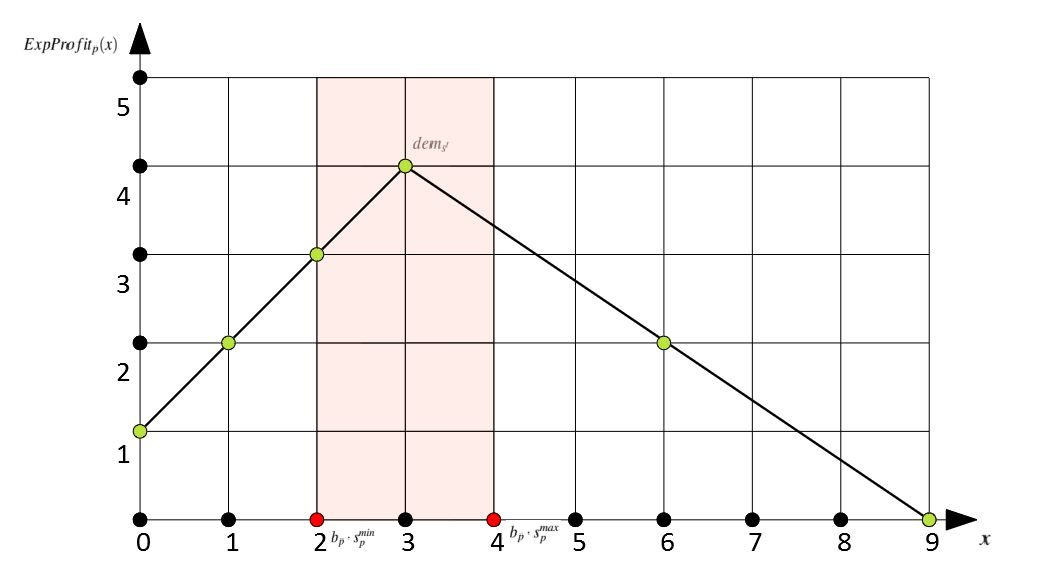
\includegraphics[scale=0.5]{expProfit_func_var}
\caption{Az optimális $x_p$ érték kiválasztásának szemléltetése}
\label{expProfit_func_var}
\end{center}
\end{figure}
\subsection{Two stage (két lépcsős ütemezés)}
Ebben az esetben $p$ termék gyártandó mennyiségét illető döntés egy bizonytalan esemény bekövetkezése után is meghozható, például, ha egy forgatókönyv már bekövetkezett. Éppen ezért a termék mennyisége az adott forgatókönyvtől függ, legyen ez: $x_{s,p}$. E mennyiség kiválasztása a következőképpen zajlik:
\begin{equation*}
x_{s,p}(b_p)= \begin{cases}
            b_p \cdot s_p^{max} \quad \text{ha } b_p \cdot s_p^{max}<dem_{s}\\
            dem_{s} \qquad \text{ha } b_p \cdot s_p^{min} \leq dem_{s} \leq b_p \cdot s_p^{max}\\
            b_p \cdot s_p^{min} \quad \text{ ha } b_p \cdot s_p^{min}>dem_{s}
       \end{cases}       
\end{equation*}\\
Látható, hogy a képlet hasonló a \ref{variable_batch_size_modell} pontban bemutatott képlethez, azonban míg ott  az $ExpProfit$ függvényből kerül kiválasztásra az optimális $x_p$ mennyiség (azaz, minden forgatókönyv esetén ez az érték ugyan annyi lesz), addig a két lépcsős ütemezés esetén minden egyes forgatókönyv $Profit$ függvényéből egyenként kerül kiválasztásra az optimális mennyiség. Ezzel megoldható az, hogy egy bizonyos forgatókönyv bekövetkezése után annak elvárásaihoz igazítsuk a termelt batch-ek méretét, jobb várható profitot elérve ezzel a legtöbb esetben. A várható profit két lépcsős ütemezés esetén a következőképpen számítható ki:
$$\sum_{p \in P} \bigg( \sum_{s \in S}(prob_s \cdot Profit(x_{s,p}(b_p)) \bigg)$$ 
\subsection{Következtetés} \label{broken_line_suggestion}
Az előzőekben bemutatott módszerek ismerete arra enged következtetni, hogy a probléma megoldásához elengedhetetlen az S-gráf keretrendszerben egy olyan osztály definiálása, amely képes  folytonos, szakaszos, lineáris függvények modellezésére, tárolására, azokon történő műveletek végrehajtására. Ezen osztály részletes leírása a \ref{broken_line_class} pontban olvasható.
\section{A BrokenLine osztály} \label{broken_line_class}
Ahogy az már korábban, a \ref{broken_line_suggestion} pontban említésre került, a probléma implementációjához elengedhetetlen egy olyan osztály definiálása, amely kezelni képes folytonos, szakaszos, lineáris függvényeket. Erre hivatott az általam megalkotott \textbf{BrokenLine} osztály, amelynek forráskódja \textbf{brokenline.h}, illetve \textbf{brokenline.cpp} fájlokban található a solver \textbf{src\textbackslash base} mappájában. Az általunk használt függvények tárolásához elegendő, ha kezdetben három pont koordinátái adottak, hiszen ezek elhelyezkedéséből a többi pont koordinátái később, ha valamilyen okból kifolyólag ez szükségessé válik, könnyen kiszámíthatóak, hiszen folytonos, lineáris függvényekről beszélünk. Ez a három pont a $profit_{s,p}$ függvények esetében nem más, mint: 
\begin{itemize}
\item $Profit_{s,p}(x)$\quad, ahol $x=dem_{s,p}-1$
\item $Profit_{s,p}(x)$\quad, ahol $x=dem_{s,p}$
\item $Profit_{s,p}(x)$\quad, ahol $x=dem_{s,p}+1$
\end{itemize} 
E három pont koordinátái minden esetben kiszámíthatók, minden forgatókönyv-termék párosra már az input fájl beolvasását követően, hiszen minden sztochasztikus paraméter adott ehhez a fájlban. Az ehhez szükséges képlet a \ref{variable_batch_size_modell} pont szerint:
\begin{equation*}
Profit_{s,p}(x)= \begin{cases}
            price_{s,p}\cdot x-(dem_{s,p}-x) \cdot uc_{s,p}\qquad \text{ha } x<dem_{s,p} \\
            price_{s,p} \cdot dem_{s,p}-(x-dem_{s,p}) \cdot oc_{s,p}\qquad \text{egyébként}
       \end{cases}
\end{equation*}
Miután ennek a három pontnak a pontos koordinátái beazonosításra kerültek, már csak annyit kell tenni, hogy kiszámítunk két arány számot, amelyek a függvény kezdeti-, és vég meredekségét hivatottak letárolni. Ezen paraméterek ismeretében később a függvény bármely $x$ pontjában felvett értéke számítható lesz. Ezek alapján a \textbf{BrokenLine} osztály adattagjai a következőek:
\begin{figure}[H]
\begin{center}
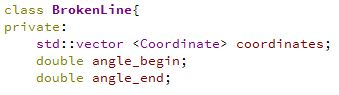
\includegraphics[scale=1]{broken_line_variables}
\caption{A \textit{BrokenLine} osztály adattagjai}
\label{broken_line_variables}
\end{center}
\end{figure} 
A \ref{broken_line_variables} ábrán látható \textbf{Coordinate} osztály a függvények pontjainak $x$ és $y$ koordinátáinak egyszerű tárolására, lekérdezésére, és összehasonlítására szolgál a megvalósított \textit{setter}, \textit{getter} és felültöltött egyenlőség operátorral.\\
Ahhoz, hogy a \textbf{BrokenLine} osztállyal a matematikai modellek minden szükséges művelete elvégezhető legyen, a következő funkcionalitást kell megvalósítani az osztálynak:
\begin{itemize}
\item Koordináta pár hozzáadása
\item Koordináta párok rendezése $x$ szerint növekvő sorrendbe
\item Kezdeti-, és vég meredekség kiszámítása
\item A függvény skalár értékkel való szorzása
\item A függvény $x$ helyen vett értékének lekérdezése
\item Két függvény összeadása
\item A függvény horizontális nyújtása (a \ref{extended_multiproduct} pontban tárgyalt esetekhez)
\item A függvény maximális értékéhez tartozó koordináták lekérdezése
\end{itemize} 
\subsection{Koordináta pár hozzáadása} \label{addCoordinates}
Egy új koordináta pár hozzáadását végző metódus az \textbf{addCoordinate(const Coordinate\& c)}. Egy új koordináta pár hozzáadása esetén először is meg kell győződnünk, hogy adott koordináta pár szerepel-e már a koordináták tárolására szolgáló vectorban, hiszen ha már szerepel, nem adhatjuk hozzá újra. Ha nem szerepel még ilyen koordináta pár, hozzáadjuk, majd rendezzük a vectort $x$ szerint növekvő sorrendbe. Ha ez megtörtént, meg kell vizsgálni, hogy a kezdeti-, és vég meredekségeket frissíteni kell-e. Abban az esetben, ha a most hozzáadott koordináta pár szerepel a rendezett vector első, vagy második helyén, a kezdeti meredekséget frissíteni kell. Hasonlóan, ha az új koordináta pár a vector utolsó, vagy utolsó előtti eleme, a vég meredekség frissítésre szorul. Mivel kezdetben akár mindkét feltétel igaz lehet, ezért ezek teljesülését két külön \textit{bool} változóban kell tárolni. Miután megállapításra került, hogy melyik meredekségeket kell frissíteni, meghívásra kerül az ezeket kiszámító függvény. 
\subsection{Kezdeti-, és vég meredekség kiszámítása} \label{calculateAngle}
A  kezdeti-, és vég meredekség kiszámítására és frissítésére hivatott metódus a \textbf{calculateAngle(bool begin,bool end)}, melynek két paramétere a \ref{addCoordinates} pontban említett két \textit{bool} változó, amelyek megadják, hogy kell e frissíteni adott meredekségeket. A meredekségek kiszámítása roppant egyszerű a koordináták ismeretében:
$$Angle_{begin}=(y_{second}-y_{first}) / (x_{second}-x_{first})$$
$$Angle_{end}=(y_{penultimate}-y_{last}) / (x_{last}-x_{penultimate})$$
A \ref{calculate angle} ábrán látható három pont koordinátái alapján a meredekségek például a következőképpen alakulnak: 
$$Angle_{begin}=(4-3) / (3-2)\quad \text{, azaz } Angle_{begin}=1$$
$$Angle_{end}=(4-2) / (6-3)\quad \text{, azaz } Angle_{end}=2/3$$
\begin{figure}[H]
\begin{center}
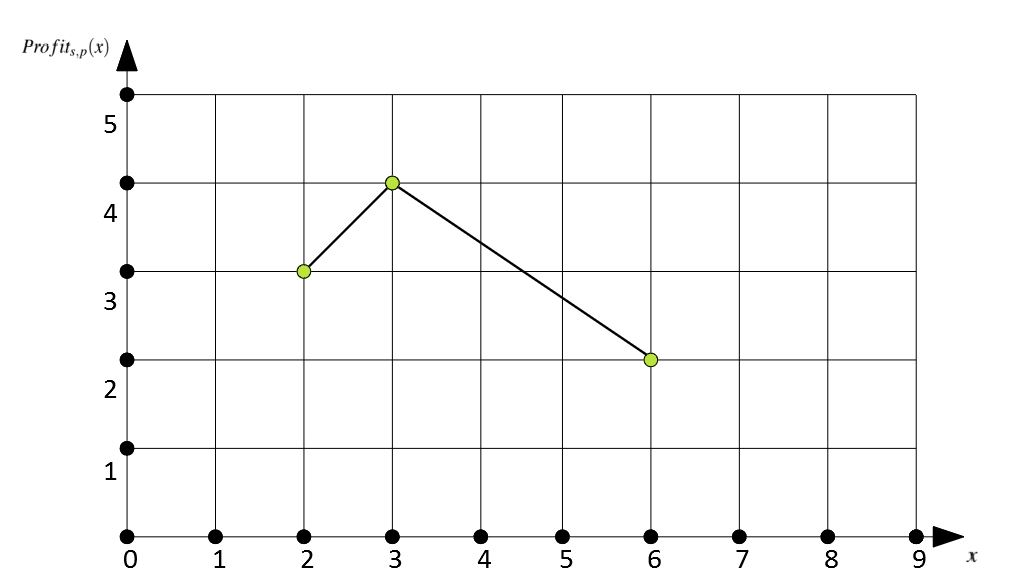
\includegraphics[scale=0.5]{calculate_angle}
\caption{Példa a meredekségek kiszámítására}
\label{calculate angle}
\end{center}
\end{figure}
Ha egyik meredekség sem szorul frissítésre, a metódus semmiféle változtatást nem tesz.
\subsection{A függvény skalár értékkel való szorzása} \label{multiplyByScalar}
A függvény skalárral való szorzását a \textbf{multiplyByScalar(double s)} metódus végzi. Ahhoz, hogy megkapjuk a függvény skalárral való szorzatát, csupán be kell szorozni a vectorban tárolt összes pont $y$ koordinátáját, valamint a kezdeti-, és vég meredekséget a paraméterként kapott $s$-el. A függvény szorzását szemléltető példa a \ref{profit_func_prob} ábrán látható.
\subsection{A függvény $x$ helyen vett értékének lekérdezése} \label{getValue}
A függvény $x$ helyen vett értékének lekérdezésére a \textbf{getValue(double x)} metódus hivatott. A metódus először is megnézi, hogy a vectorban tárolt koordináta párok között található-e olyan, amelynek $x$ koordinátája egyezik a paraméterként kapott $x$-el. Ha talál ilyet, egyszerűen visszaadja a megfelelő koordináta párost tartalmazó \textbf{Coordinate} objektumot. Ha nem található ilyen pont, akkor annak ki kell számítani a koordinátáit, és hozzá kell adni a vectorhoz, majd csak ezután lehet visszaadni a keresett \textbf{Coordinate} objektumot. Az $x$ értékhez tartozó $y$ érték kiszámítása a keresett $x$ értéke és a vectorban tárolt pontok alapján háromféleképpen történhet:
\begin{itemize}
\item Ha a keresett $x$ értéke kisebb mint a vectorban tárolt első pont $x$ koordinátájának értéke, akkor: 
$y=y_{First}-(x_{First}-x) \cdot Angle_{begin}$ ,ahol $x_{First} \text{ és } y_{First}$ a vectorban tárolt első pont koordinátái.
\item Ha a keresett $x$ érték két a vectorban tárolt pont $x$ koordinátájának értéke közé esik, akkor:
$y=\bigg(\big(x-x_{LastSmaller}\big) \cdot \big((y_{FirstBigger}-y_{LastSmaller})/(x_{FirstBigger}-x_{LastSmaller})\big)\bigg)+y_{LastSmaller}$ ,ahol $x_{LastSmaller} \text{ és } y_{LastSmaller}$ a keresett $x$ értéket megelőző pont koordinátái, míg $x_{FirstBigger} \text{ és } y_{FirstBigger}$ a keresett $x$ értéket követő pont koordinátái. 
\item Ha a keresett $x$ értéke nagyobb, mint a vectorban tárolt utolsó pont $x$ koordinátájának értéke, akkor:
$y=y_{Last}-(x-x_{Last}) \cdot Angle_{end}$ ,ahol $x_{Last} \text{ és } y_{Last}$ a vectorban tárolt utolsó pont koordinátái.
\end{itemize}
\subsection{Két függvény összeadása} \label{addBrokenLine}
Két függvény összeadását az \textbf{addBrokenLine(BrokenLine b)} metódus végzi, melynek visszatérési értéke az összegként kapott függvényt tároló új \textbf{BrokenLine} objektum. Mivel a függvények tárolásához elegendő három pont tárolása, ezért gyakran előfordul olyan eset, hogy a két összeadni kívánt \textbf{BrokenLine} objektum nem tartalmazza a szükséges koordinátákat, ezért a hiányzó koordináta párokat először hozzá kell adni, ezt azonban megkönnyíti a \ref{getValue} pontban bemutatott \textbf{getValue} metódus, hiszen elég, ha lekérdezzük az aktuális $x$ értékét mindkét függvény esetén, és ha az valamelyiknél nem található, automatikusan hozzá lesz adva annak pontjaihoz. Ennek következtében a két függvény összeadása már jóval egyszerűbb feladat, egyetlen \textit{for} ciklussal megtehető.
\begin{figure}[H]
\begin{center}
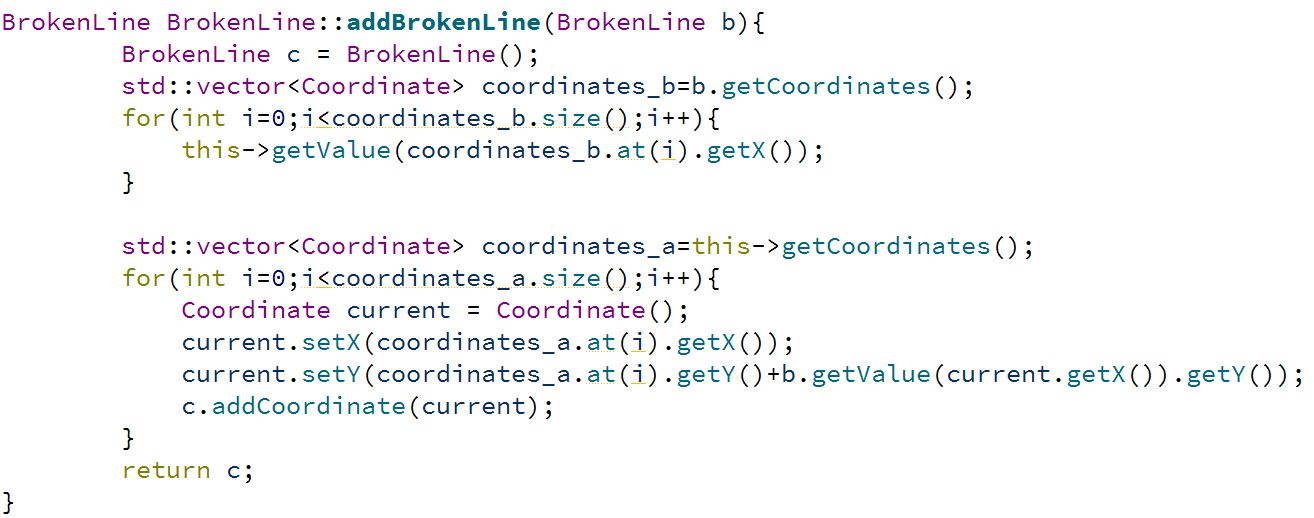
\includegraphics[scale=0.48]{add_broken_line}
\caption{Az \textit{AddBrokenLine} metódus}
\label{add_broken_line}
\end{center}
\end{figure}
\subsection{A függvény horizontális nyújtása}
A függvény a \ref{extended_multiproduct} pontban használt horizontális nyújtását (illetve összenyomását, s értéktől függően) a \textbf{stretchHorizontally(double s)} metódus végzi. A metódus egyszerűen egy \textit{for} ciklus segítségével a függvény összes pontjának $x$ koordinátáját, valamint a kezdeti-, és vég meredekséget beszorozza a paraméterként kapott $s$ értékkel, illetve a meredekségek esetén annak reciprokával.
\begin{figure}[H]
\begin{center}
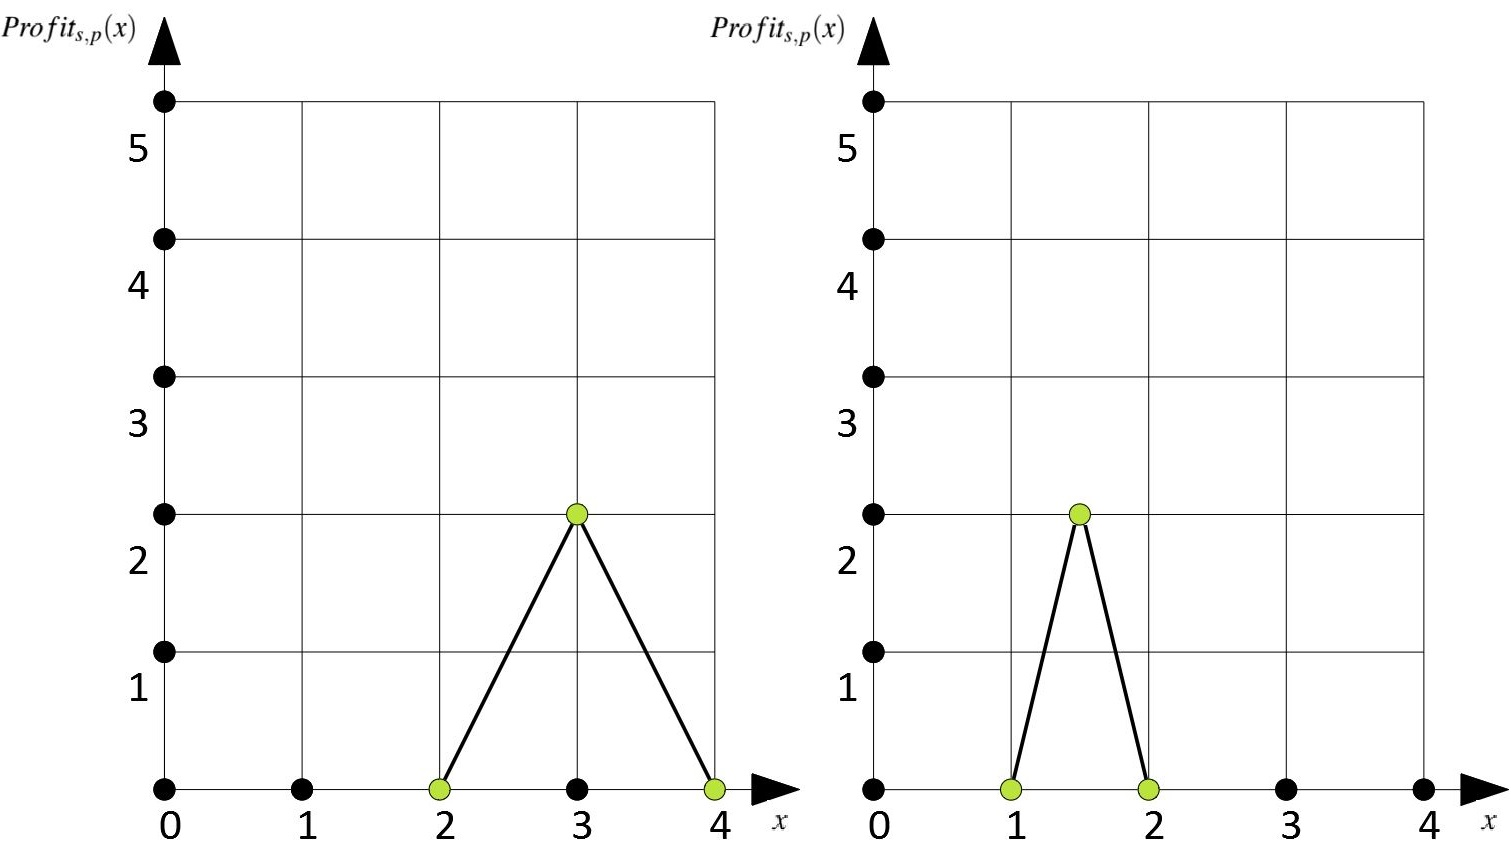
\includegraphics[scale=0.5]{profit_func_stretch}
\caption{Példa a függvény horizontális nyújtására $s=0.5$ értékkel}
\label{profit_func_stretch}
\end{center}
\end{figure}
\subsection{A függvény maximális értékéhez tartozó koordináták lekérdezése}
A függvény maximumának lekérdezését a \textbf{getMaximum()} metódus végzi, mely egy egyszerű maximum keresést valósít meg $y$ koordinátára nézve. A metódusnak a \ref{variable_batch_size_modell} pontban bemutatott változó batch méretű esetben van nagy jelentősége, ezt használjuk ugyanis $dem_{s'}$ meghatározására.
\section{Az új paraméterek implementációja}
Ahhoz, hogy az általános throughput maximalizáló használható legyen a \ref{problem_parameters} pontban bemutatott új sztochasztikus paraméterekkel, fel kell készíteni a megfelelő osztályokat ezen paraméterek kezelésére, be kell olvasni először is ezeket a paramétereket egy input fájlból, majd valamilyen formában le is kell őket tárolni, hogy később a \ref{math_modells} pontban bemutatott műveletek végrehajthatóak legyenek a várható profit kiszámítására.
\subsection{Új kapcsoló definiálása}
Mivel a sztochasztikus throughput maximalizáló működhet preventív, illetve két lépcsős módon, ezért szükségessé vált egy új parancssori kapcsoló bevezetése:
\begin{figure}[H]
\begin{center}
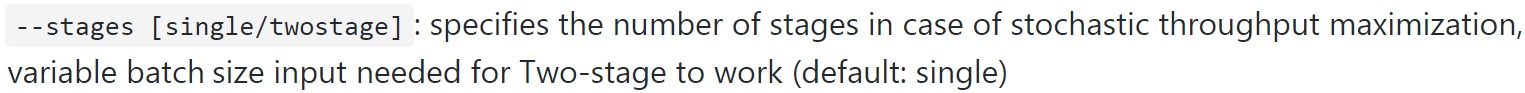
\includegraphics[scale=0.65]{switch}
\caption{Az új kapcsoló leírása a readme fájlban}
\label{switch}
\end{center}
\end{figure}
Abban az esetben, ha nem adjuk meg a kapcsoló értékét, vagy azt single-re állítjuk, preventív módban fog futni az ütemező, ha twostage-t állítunk be, két lépcsős ütemezés fog lefutni, feltéve, hogy a bemeneti fájlban változó batch méretű adatokat adtunk meg.
\subsection{Új input fájl definiálása}
Az általam definiált új input fájl a \textbf{stochastic.ods} a solver \textbf{input} mappájában található. A fájl lényegében a \textbf{multipurpose.ods} kibővítése a sztochasztikus paraméterekkel, éppen ezért az utóbbi \textbf{equipment}, és \textbf{proctime} tábláit változtatás nélkül tartalmazza, hiszen ezek tartalmazzák a gépekre, illetve a recept gráfra vonatkozó determinisztikus paramétereket, amelyeket az új esetekben is fel kell használnia a megoldó algoritmusnak. Ezzel szemben a \textbf{product} tábla a sztochasztikus esetekben nem fogja megállni a helyét, hiszen a batch méretekre vonatkozó adatok hiányoznak belőle, ezeket hozzá kell adni a product táblához. Ezenkívül a forgatókönyvek adatait is tárolnunk kell, ezért bevezetésre kerültek a\textbf{ scenario}, és a \textbf{scenario\_data} táblázatok, melyek a \ref{problem_parameters} pontban leírt, forgatókönyvekre vonatkozó sztochasztikus adatokat tartalmazzák. A példa input fájlok megtekinthetőek a \textbf{\ref{input_files}} függelékben.
\subsection{A beolvasott paraméterek tárolása}
\section{Szükséges változtatások az általános throughput maximalizálón} \label{refactor}
\subsection{A meglévő kód refaktorálása}
\subsection{A \textit{getRevenue()} metódus}
\section{Multiproduct receptek esete} \label{extended_multiproduct}